\chapter{绪论} 
\thispagestyle{others} 
\pagestyle{others} 
\xiaosi 

\section{研究背景及意义}
随着大数据时代的到来和人工智能技术的迅猛发展,数据资源已成为驱动各行各业决策能力和服务质量提升的战略要素。数据隐私保护法规日益严格,使得不同机构之间的数据协作面临着前所未有的挑战,极大地限制了数据价值的深度挖掘。在此背景下,联邦学习\textsuperscript{\cite{chen2021secureboost+,de2010practical}}作为一种新兴的分布式机器学习方法应运而生。它允许多个数据拥有方在不共享原始数据的前提下,通过交换模型参数或梯度信息实现模型的联合训练,成功解决了数据隐私保护与联合建模之间的矛盾。在联邦学习的众多研究方向中,纵向联邦学习(Vertical Federated Learning, VFL)因其能够有效整合不同机构所拥有的互补特征数据而得到广泛关注,并被广泛应用于金融、医疗、推荐系统等领域\textsuperscript{\cite{liu2020secure,chen2020vafl}}。目前VFL主要集中于监督学习领域,严重依赖大量的标记和对齐数据。在实际应用中,VFL往往面临标注成本高、领域专家稀缺、资源受限以及对齐样本不足等挑战,导致大量潜在有用数据无法被有效利用,进而制约了模型泛化能力与应用效果的提升\textsuperscript{\cite{li2021comatch}}。在现实应用中常常只有一方拥有标签信息,这进一步加剧了联合模型训练的复杂性。如何高效利用未完全标记数据和未对齐样本成为当前VFL领域亟待解决的难题。

针对上述问题,本文提出了一种结合VFL与PU学习(Positive and Unlabeled Learning, 正例和无标签学习)\textsuperscript{\cite{pulearn}}的方法(Vertical Federated learning with Positive and Unlabeled data,VFPU)。该方法有效解决了未标记数据缺失所带来的PU学习挑战,即未标记数据缺失的PU学习问题(Unlabeled-Data-Deficient PU, UDD-PU)。本文进一步提出一种基于联邦半监督学习的参与方样本生成方法(Participants Sample Generation method based on VFPU-Multitask, FedPSG-PUM),通过融合半监督学习与数据生成技术,在不共享原始数据和模型参数的前提下,实现对未对齐样本的高效利用。具体而言,VFPU方法允许多方在保护数据隐私的前提下,融合PU学习策略,实现半监督学习模型的协同训练。该方法有效弥补了现有VFL框架过度依赖大量标记数据的缺陷,进一步拓宽了PU学习在真实业务场景中的应用范围。FedPSG-PUM方法则通过分析特征间相关性、伪标签预测和表格数据生成,有效解决了VFL中样本对齐不足的难题,提高了数据资源的利用效率和模型的泛化性能。这些方法的提出不仅在理论上拓展了联邦学习与半监督学习的研究范畴,也为金融风险控制、医疗诊断与疾病预测、智能制造预测性维护以及智能推荐系统等领域存在的数据孤岛问题提供了切实可行的解决方案。

%它们有助于各行业在确保数据隐私安全的前提下,更加精准地进行数据驱动决策,同时为联邦学习场景中的复杂半监督学习问题提供了有力的理论支持和实践指导。



\section{国内外研究现状}
本节将从联邦半监督学习和数据生成方法两个方面综述国内外研究进展,分析现有方法的优势与不足,后文提出的联邦半监督学习框架与样本生成方法奠定理论基础。
\subsection{联邦半监督学习}
在联邦半监督学习的应用中,根据标记数据的位置的不同,通常可以将其分为两种情况:标签存储在客户端,即每个参与方仅拥有自己数据的标记信息;标签存储在服务器端,在这种情况下,服务器负责汇总所有标记信息并协调各参与方的学习过程。这两种技术架构在实际应用中各有优劣,涉及的技术细节和隐私保护策略也有所不同。随着越来越多的应用场景对数据隐私的要求日益严格,如何有效地进行半监督学习,特别是在联邦学习框架下,在确保数据隐私的同时提升模型性能,已成为当前研究的热点之一\textsuperscript{\cite{jin2023federated}}。

(1) 标签在客户端

标记数据存储于客户端,而服务器只能获取未标记数据。例如,某家公司欲利用智能手机拍摄的图片训练一个物体检测的联邦学习模型,但无法直接访问用户的本地数据,只能依赖用户的标注,如图 \ref{LabelAtClient} 所示。对于不同的参与方(用户),样本ID是不同的,但参与方(用户)手机里的图片特征是一样的。用户通常不愿为每张照片标注,创造了一个标签在客户端(label-at-client)的环境。基于这一场景,研究者们提出了多种联邦半监督学习方法,下面将对这些方法进行介绍。

\vspace{-0.1cm}
\begin{figure}[h]
	\centering
	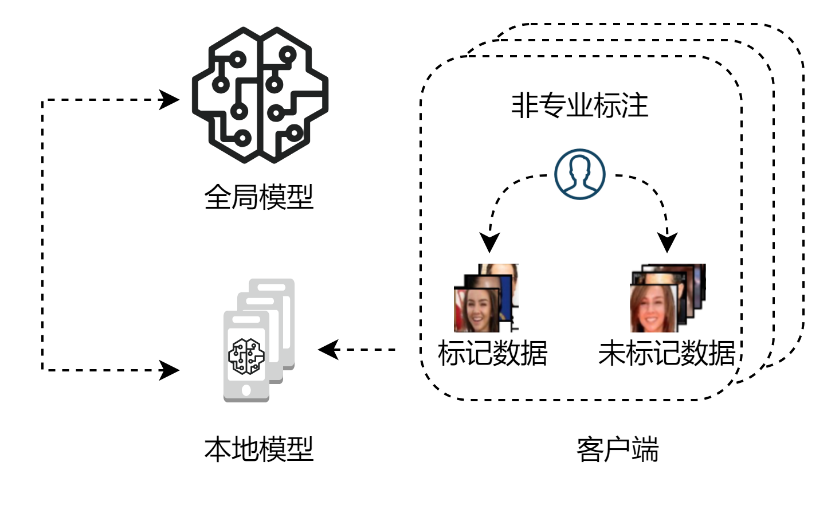
\includegraphics[width=10cm]{chapters/imgs/LabelAtClient}
	\bicaption[\xiaosi 标记数据在客户端的情况]
	{\wuhao 标记数据在客户端的情况}
	{\wuhao Labeled data on the client side}
	\label{LabelAtClient}
\end{figure}
\vspace{-0.35cm}

LIANG等人\textsuperscript{\cite{liang2022rscfed}}提出了随机采样共识联邦半监督学习(Random Sampling Consensus Federated Semi-Supervised Learning, RSCFed),通过将多个子集模型聚合与距离加权策略相结合,缓解了标签隔离与数据异质性问题。随后,FAN 等人\textsuperscript{\cite{fan2022private}}提出了私有联邦半监督学习(Private Semi-Supervised Federated Learning, FedSSL),利用伪标签与差分隐私机制进一步解决了未标注客户端的训练需求与潜在的隐私泄露风险。而针对在客户端间建立一致性损失以缓解数据分布不一致问题,ZHENG 等人\textsuperscript{\cite{jeong2020federated}}则提出了联邦匹配(Federated Match, FedMatch),通过在各客户端与其邻近客户端之间增加一致性约束来提升模型鲁棒性。为更好地在服务器端利用未标记数据并在效率与准确性之间取得平衡,WANG 等人\textsuperscript{\cite{wang2022enhancing}}提出了增强型联邦半监督学习(Enhancing Federated Learning with In-Cloud Unlabeled Data, AdaFedSemi),通过自适应地调整客户端参与率与伪标签阈值改善了全局模型性能与通信成本。为了在服务器端未标记数据的基础上实现更高效的协同训练,ITAHARA 等人\textsuperscript{\cite{itahara2021distillation}}开发了基于蒸馏的联邦半监督学习(Distillation-based Semi-Supervised Federated Learning, DS-FL),使用多客户端伪标签平均生成的集合标签来提升模型泛化能力。最后,对于一个更具挑战性的半监督学习设置,即PU学习设置,Lin 等人\textsuperscript{\cite{FedPU}}提出了联邦PU学习(Federated Positive and Unlabeled Learning, FedPU)方法,推导出了一种新的目标函数,使得学习客户端的负类任务可以转交给其他在负类上有标签数据的客户端。通过这种方式,每个客户端只需要负责学习正类,并且可以独立进行本地训练。

\vspace{-0.1cm}
\begin{figure}[h]
	\centering
	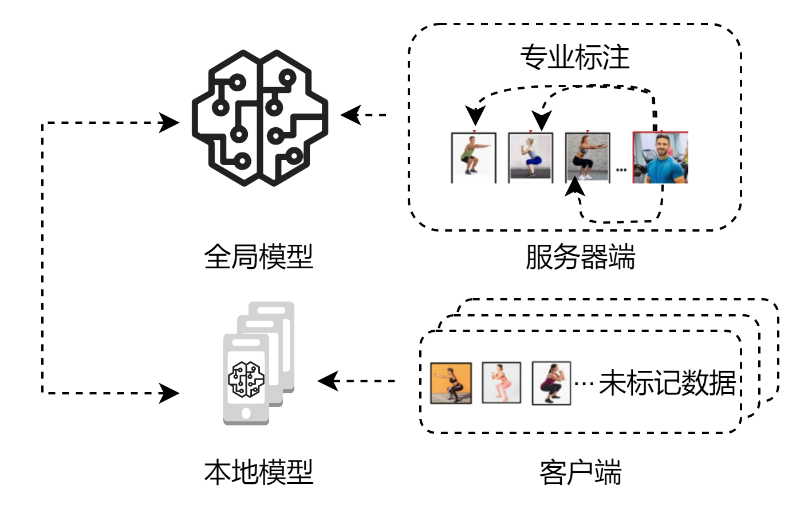
\includegraphics[width=10cm]{chapters/imgs/LabelAtServer}
	\bicaption[\xiaosi 标记数据在服务端的情况]
	{\wuhao 标记数据在服务端的情况}
	{\wuhao Labeled data on the server side}
	\label{LabelAtServer}
\end{figure}
\vspace{-0.35cm}

(2) 标签在服务器端

标记数据存储于服务器,而客户端只有未标记数据。例如,一家可穿戴设备公司希望利用联邦学习训练健康监测模型,如图 \ref{LabelAtServer} 所示。在这种情况下,由于用户通常缺乏专业知识,无法标注健康相关数据,因此客户端的数据是未标记的。标签数据在服务端的情况比标签在客户器端更复杂,原因是所有客户端都只拥有未标记数据,无法为联邦模型提供额外的监督信号,仅使用无标签数据进行训练可能会导致遗忘从有标签数据中学到的知识,从而影响模型性能\textsuperscript{\cite{jeong2020federated,diao2022semifl}}。


为了解决标签数据和非标签数据之间的隔离问题,ZHENG 等人\textsuperscript{\cite{jeong2020federated}}提出了一种不相干的学习方案,即分别为标签数据和非标签数据设置一套参数。在非标签数据上进行训练时,标签数据的参数是固定的,以防止知识被覆盖。非标记数据的参数会在参与者和服务器之间传输,而非标记数据的参数设置为稀疏的,这为通信效率带来了额外的好处。此外,为了解决不同客户端持有的异构数据问题,ZHENG 等人\textsuperscript{\cite{jeong2020federated}}提出了客户端间一致性损失,这样不同参与者的本地模型就能在相同数据上产生相似的输出。

\vspace{-0.1cm}
\begin{table}[h]
	\centering
	\bicaption[\xiaosi \songti 联邦半监督学习方法总结]
	{\songti \wuhao 联邦半监督学习方法总结}
	{\songti \wuhao Summary of federated semi-supervised learning methods}
	\label{SummaryOfFedSemi}
	\resizebox{\textwidth}{!}{
		{\songti \wuhao
			\begin{tabular}{cccccc}
				\toprule[1.5pt]
				类别 & 方法 & 半监督学习算法 & 隐私保护方案 & 数据异质问题 & 性能 \\
				\midrule
				\multirow{6}{*}{标签在客户端} 
				& RSCFed     & 教师学生模型 & 无     & 加权距离聚合   & 无                \\
				& FedSSL     & 伪标记       & 差分隐私 & 全局生成模型     & 无               \\
				& FedMatch   & 伪标记       & 无     & 客户端间一致性  & 分散学习和稀疏学习 \\
				& FedPU      & PU Learning  & 无     & 客户端间一致性  & 无                \\
				& AdaFedSemi & 伪标记       & 无     & 无             & 调整置信度阈值和参与率 \\
				& DS-FL      & 集成未标记   & 无     & 无             & 传输日志、无参数     \\
				\midrule
				\multirow{2}{*}{标签在服务器端} 
				& SemiFL     & 伪标记       & 无     & 减少熵的平均值   &                   \\
				& FedMatch   & 伪标记       & 无     & 客户端间一致性   & 分散学习和稀疏学习   \\
				\bottomrule[1.5pt]
			\end{tabular}
		}
	}
\end{table}
\vspace{-0.35cm}

DIAO 等人\textsuperscript{\cite{diao2022semifl}}提出了半监督联邦学习方法(Semi-supervised Federated Learning, SemiFL),为应对上述挑战提供了另一种思路。该方法首先利用带标注数据对全局模型进行微调,从而提升模型质量并减轻因客户端无监督训练而带来的遗忘现象;同时,该方法主张增强客户端模型与全局模型间的一致性,而非在客户端之间对模型输出进行正则化。

(3) 联邦半监督学习方法总结

表 \ref{SummaryOfFedSemi} 总结了前文介绍的基于联邦的半监督学习方法,按照标签在客户端或服务器端进行划分。从表中可以看出,这些方法在半监督学习算法、隐私保护方案、数据异质问题和性能提升策略方面存在着差异。当标签位于客户端时,这些方法主要采用教师学生模型、伪标记和PU学习等半监督学习算法,其中FedSSL方法通过差分隐私来保护数据隐私,FedMatch则强调客户端间的一致性,AdaFedSemi则通过调整置信度阈值和客户端参与率来提高模型性能。当标签位于服务器端时,SemiFL 和 FedMatch 方法分别通过伪标记算法增强客户端模型与全局模型的一致性,且都没有额外的隐私保护措施。SemiFL 通过减少熵的平均值来提升全局模型质量,减轻客户端无监督训练带来的遗忘问题;而 FedMatch 强调客户端间的一致性,采用分散学习和稀疏学习策略来优化模型性能。



\subsection{数据生成方法}
生成合成数据的主要策略集中在生成模型上,这些模型旨在从现有数据集中学习丰富的表示,并随后生成新的样本。目前,这些方法已在医学研究、金融、教育等多个领域得到广泛应用。在这些领域中,生成高质量的合成数据意义重大,它不仅有助于保护数据隐私,还能对有限的数据集进行有效扩充。以下将对常见的数据生成方法进行详细介绍。

基于自编码器的方法:这一类别中的先驱性工作是自编码器(Autoencoder, AE)\textsuperscript{\cite{hinton2006reducing}},其训练目的是将高维输入映射到低维潜在编码中,然后从这些编码中重构原始数据。通过强制隐藏(潜在)层降维,AE有效地学习到了压缩表示。然而,纯粹的AE是确定性的,缺乏灵活采样的直接机制。变分自编码器(Variational Autoencoder, VAE)\textsuperscript{\cite{kingma2013auto}} 通过引入概率潜在变量框架解决了这一问题,从而可以从学习到的潜在分布中采样出新的、未见过的数据点。这一扩展极大地拓宽了基于自编码器模型在合成数据生成中的潜在应用范围。在 AE 和 VAE 的基础上,XU 等人\textsuperscript{\cite{xu2019modeling}} 提出一种针对表格数据生成与重构的改进方法。该方法能够更加准确地建模潜在变量与表格特征(包括连续与离散属性)的联合分布,从而提升对混合类型数据的生成质量。通过关注不同类型变量之间的相互作用,该方法确保生成的合成数据忠实地反映了真实世界表格数据集(如医疗和教育数据)中存在的复杂依赖关系。

基于生成对抗网络(Generative Adversarial Networks, GANs)\textsuperscript{\cite{goodfellow2014generative}}的方法:自2014年引入以来,GANs对生成建模领域产生了重大影响。其基本概念基于博弈论:两个网络——生成器(Generator, G)和判别器(Discriminator, D)——在对抗循环中训练。判别器学习区分真实数据和合成数据,而生成器则试图生成能够欺骗判别器的样本。当判别器无法再区分真实数据与生成数据时,这个极小极大博弈就告一段落,这表明生成器已经捕捉到了底层分布的统计特征。在GANs出现后不久,MIRZA等人\textsuperscript{\cite{mirza2014conditional}} 提出了条件生成对抗网络(Conditional Generative Adversarial Networks, CGANs),其中生成器和判别器均基于辅助信息(如类别标签或特定输入变量)进行条件化。这一扩展框架使得生成能够针对特定类别或属性进行定向,实际上将原本的无监督设置转变为有监督或半监督范式。尽管取得了这些进展,传统GANs往往仍然面临梯度消失或模式崩溃的问题。为了解决这些问题,Banach等人用Wasserstein距离替换了Jensen–Shannon(JS)和Kullback–Leibler(KL)散度,从而诞生了Wasserstein GAN(WGAN)\textsuperscript{\cite{adler2018banach,arjovsky2017towards}}。

针对表格数据的GANs:虽然GANs最初因图像合成而受到欢迎,但它们在处理通常具有异构特征类型、不平衡和复杂依赖关系的表格数据集时,同样证明既具有挑战性又极具价值。针对这些挑战,LIU等人\textsuperscript{\cite{xu2018synthesizing}} 提出了表格GAN(Table GAN, TGAN),该方法在生成器网络中应用了长短期记忆单元,并在判别器中采用了多层感知器,从而使深度架构适应于表格数据生成(例如健康记录或学生成绩数据)。2019年,XU等人\textsuperscript{\cite{xu2019modeling}}提出了CTGAN(Conditional Table GAN),一种专门为处理不平衡离散列、多模态连续列以及表格数据固有复杂性而设计的改进型条件GAN架构。CTGAN 凭借其条件采样策略,在对数据的精细分布进行建模以及生成与真实数据高度匹配的表格行方面展现出了优异表现。

表格GANs进一步发展,LEE等人\textsuperscript{\cite{lee2021invertible}}探索了一种可逆的表格GAN框架,该框架将对抗训练与来自可逆神经网络的负对数密度正则化相结合。该方法在训练过程中增加或降低真实样本的对数密度,从而根据隐私和质量目标生成更接近或更远离真实数据流形的合成样本。为了解决模式崩溃的问题并提高样本多样性,NGUYEN等人\textsuperscript{\cite{nguyen2017dual}}提出了一种双判别器GAN,该方法结合了KL散度和反向KL散度,以更好地捕捉真实世界数据分布的多模态特性。SINGH等人\textsuperscript{\cite{singh2021metgan}} 针对内存限制问题提出了MeTGAN,在生成器和判别器中采用稀疏线性层,从而显著降低了内存开销,而对合成质量影响不大,这在处理具有高基数类别变量的表格数据集时尤为有利。在扩展CTGAN功能方面,ZHAO等人\textsuperscript{\cite{zhao2021ctab}} 提出了CTAB-GAN,能够对连续、离散和混合类型的特征进行建模。该方法能够有效处理偏态分布和多样化的特征类型,通常在与真实数据的相似性和下游任务准确性方面优于其他基线方法。%Engelmann最后,通过在真实数据集上的实验验证,系统评估所提方法的有效性和优越性,并分析其在隐私保护、数据异构性处理和性能优化方面的表现。

\section{论文研究的主要内容}
本论文针对纵向联邦中未标记样本缺失以及对齐样本不足的问题开展研究,具体的研究内容和解决方案包括:

(1)研究未标记样本缺失的PU问题

针对VFL场景中仅含正样本和未标记样本的半监督学习问题,特别关注了未标记数据缺失的PU学习(UDD-PU)挑战,研究了一种结合VFL与PU学习的方法——VFPU。该方法在保护数据隐私的基础上,通过安全交换加密后的中间计算结果实现了多方协作训练,同时有效地利用PU学习策略深入挖掘未标记数据的潜在价值,以提升分类模型性能。研究中定义并分析了UDD-PU问题,阐述了VFPU的具体框架与算法流程,并通过实验验证了其在多个真实数据集上的有效性。该方法对解决实际应用中数据孤岛与隐私保护的挑战具有重要意义,适用于金融、医疗和智能制造等多个领域。

(2)研究对齐样本不足的问题

针对VFL中普遍存在的样本对齐不足的问题,研究了一种基于联邦半监督学习的参与方样本生成方法——FedPSG-PUM。该方法利用半监督学习策略,结合特征相关性,提出了一种创新的多任务框架,以有效提升联邦学习的性能。当特征相关性较高时,方法使用伪标签预测扩展训练集;当特征相关性较低时,则采用生成模型合成缺失特征数据。FedPSG-PUM方法通过在增强的数据视图上联合训练多个分类器,改善模型整体表现。此外,该方法在整个过程中确保参与方不交换原始数据或模型参数,严格保护数据隐私。本章还对问题进行了详细定义和分析,并通过多个真实数据集实验验证了方法的有效性。

\section{论文组织结构}
本文主要研究联邦半监督学习方法及其在样本生成中的应用,旨在解决多方数据协作中的标记数据稀缺和对齐样本不足等问题。全文分为五个章节,具体内容安排如下:


第1章为绪论。该章首先将本文的研究背景和意义进行了描述,之后大致介绍了其研究现状,最后介绍了本文的主要工作。

第2章为相关理论介绍。该章介绍了研究相关的基础理论,包括联邦学习的基本概念、分类及隐私保护应用,半监督学习的核心思想与方法,及表格数据生成技术的原理与应用。

第3章为基于多方联邦的半监督学习方法研究。本章聚焦于多方联邦学习中未标记数据缺失的问题,提出了VFPU算法。首先分析了未标记数据缺失问题(UDD-PU)的定义与特性,随后详细介绍了VFPU算法的框架设计及其在多方联邦环境下的实现流程。通过在多个数据集上的实验验证,展示了VFPU在推荐任务中的优越性能,并对实验结果进行了深入分析,最后总结了本章的研究贡献与局限性。

第4章为基于联邦半监督学习的参与方样本生成方法。该章针对纵向联邦学习中对齐样本不足的挑战,提出了FedPSG-PUM方法。本章首先分析了问题的定义与场景假设,随后系统阐述了FedPSG-PUM的整体框架,包括跨方特征相关性计算、半监督预测和生成模型合成三个核心流程,并对算法设计与实现细节进行了详细描述。通过多组实验验证了该方法在性能提升和隐私保护方面的有效性,并对结果进行了全面分析,最后总结了本章工作的创新点与应用价值。

第5章为总结与展望。该章对全文研究内容进行了归纳总结,提炼了基于联邦半监督学习的样本生成方法的核心成果与贡献,分析了所提方法的理论意义和实践价值。同时,针对研究中存在的不足之处,提出了未来工作的改进方向。
\clearpage




